% LaTeX source for ``การเรียนรู้ของเครื่องสำหรับเคมีควอนตัม (Machine Learning for Quantum Chemistry)''
% Copyright (c) 2022 รังสิมันต์ เกษแก้ว (Rangsiman Ketkaew).

% License: Creative Commons Attribution-NonCommercial-NoDerivatives 4.0 International (CC BY-NC-ND 4.0)
% https://creativecommons.org/licenses/by-nc-nd/4.0/

\chapter{การเรียนรู้แบบไม่มีผู้สอน}
\label{ch:unsup_ml}

\begin{figure}[H]
    \centering
    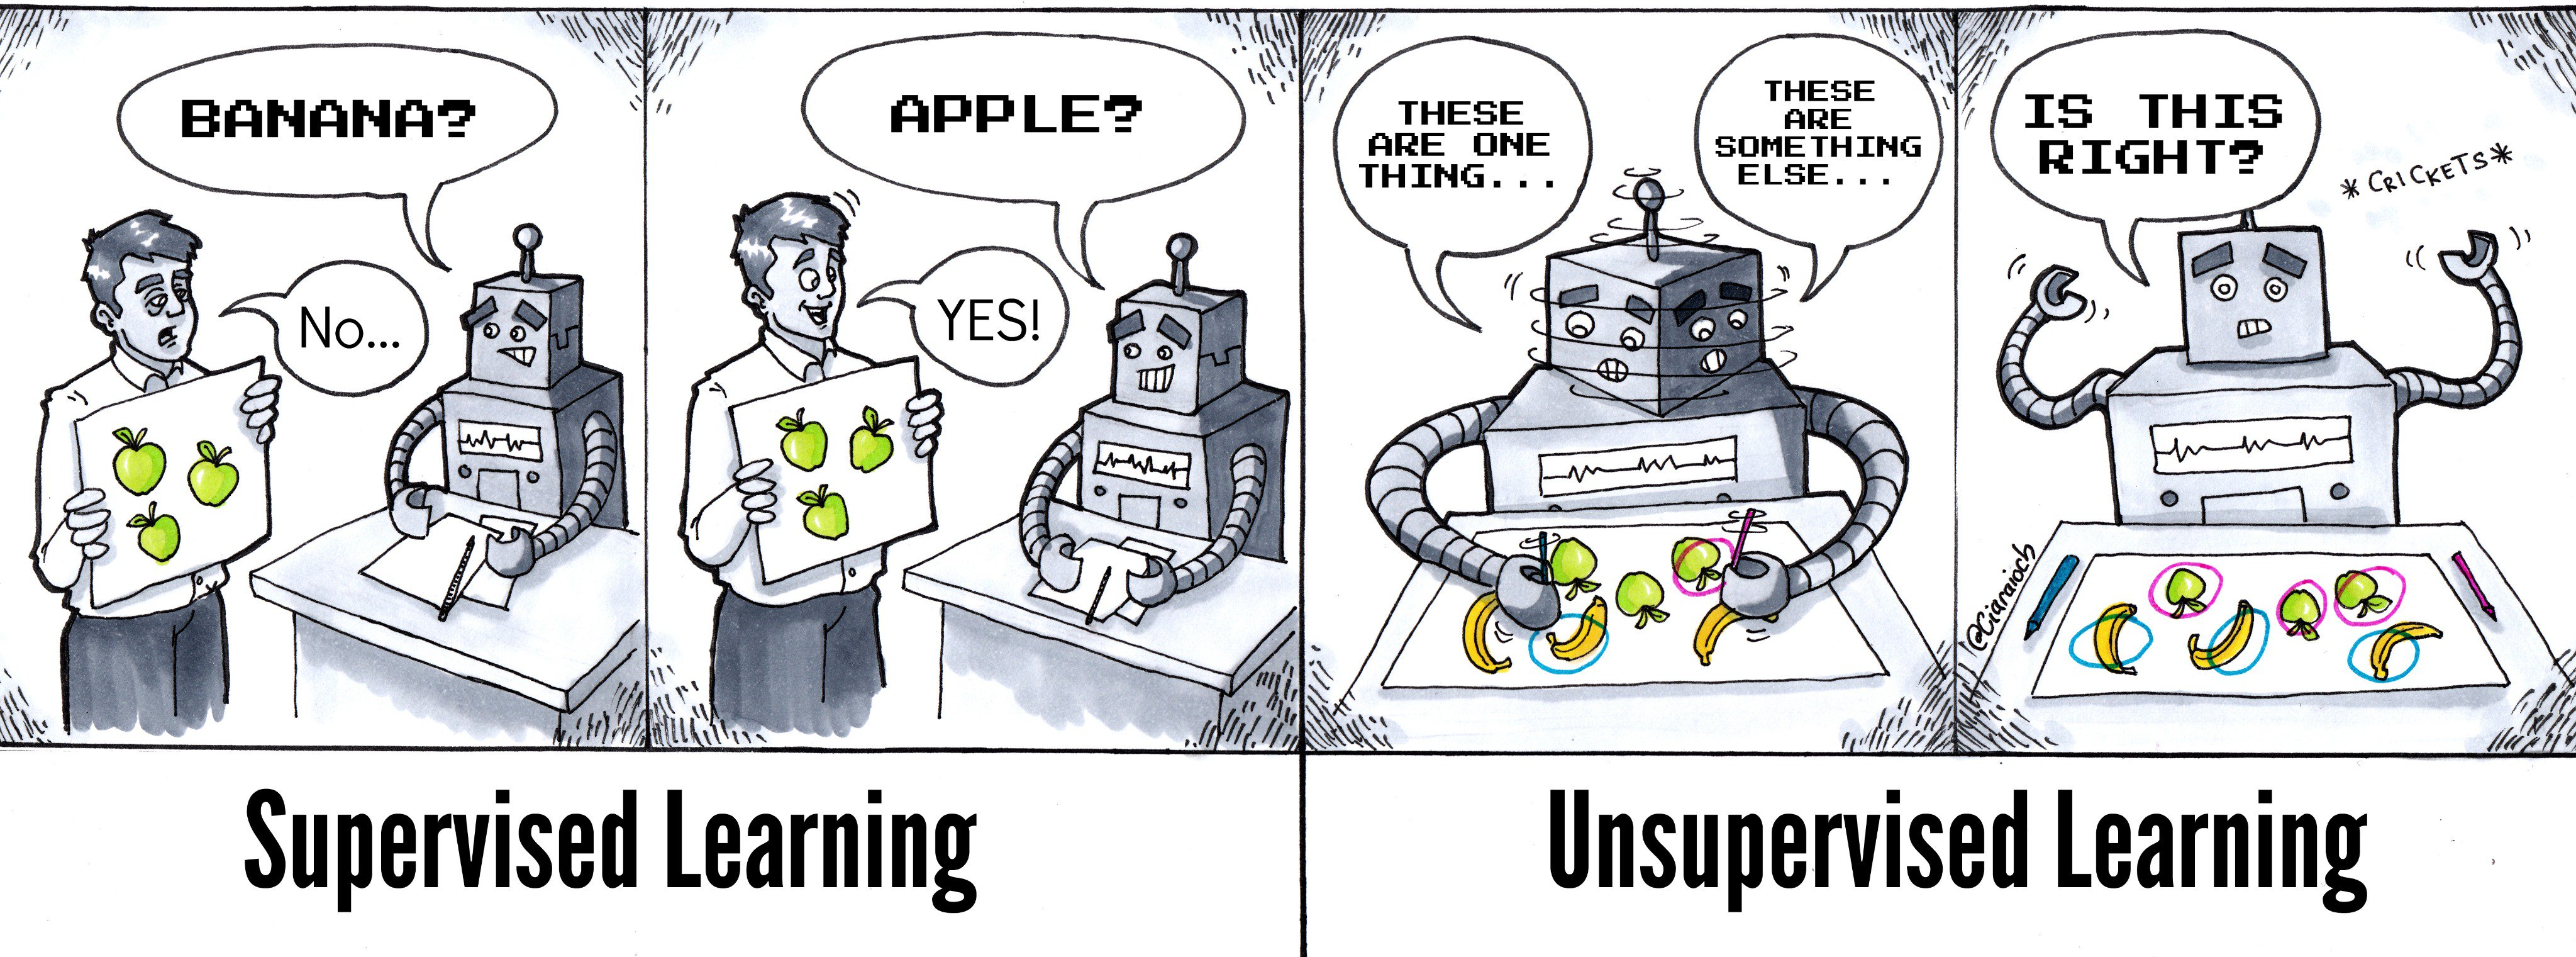
\includegraphics[width=0.9\linewidth]{fig/sup_vs_unsup_ml.jpeg}
    \caption{การเปรียบเทียบระหว่างการเรียนรู้แบบมีผู้สอน (Supervised Learning) และการเรียนรู้แบบไม่มีผู้สอน (Unsupervised Learning) ของเครื่องจักร (เครดิตภาพ: https://twitter.com/Ciaraioch)}
    \label{fig:sup_vs_unsup_ml}
\end{figure}

การเรียนรู้แบบไม่มีผู้สอน (Unsupervised Learning) เป็นเทคนิคที่อาจจะเรียกว่าได้ตรงข้ามกับการเรียนรู้แบบมีผู้สอน (Supervised Learning) ก็ได้ เพราะว่าเทคนิคประเภทนี้จะเป็นการฝึกสอนโมเดลแบบไม่มีการบอกคำตอบหรือเอาต์พุตให้โมเดลได้รับรู้ ดังนั้นสิ่งที่โมเดลมีอย่างเดียวก็คืออินพุต ซึ่งสิ่งเดียวที่โมเดลจะทำได้นั่นก็คือการเรียนรู้หาความสัมพันธ์ (Relation) ระหว่างข้อมูลแต่ละตัวภายในชุดข้อมูลที่เราได้ป้อนเข้าไป การเรียนรู้ประเภทนี้จะพิจารณาข้อมูลเป็นเซตของตัวแปรสุ่ม แล้วจึงสร้างโมเดลความหนาแน่นร่วมของชุดข้อมูล การเรียนรู้แบบไม่มีผู้สอนสามารถนำไปใช้ร่วมกับการทฤษฎีของเบย์ (Bayes' theorem) เพื่อหาความน่าจะเป็นแบบมีเงื่อนไขของตัวแปรสุ่มโดยกำหนดตัวแปรที่เกี่ยวข้องให้ นอกจากนี้ยังสามารถนำไปใช้ในการบีบอัดข้อมูล (Data Compression) ซึ่งขั้นตอนวิธีการบีบอัดข้อมูลจะขึ้นอยู่กับการแจกแจงความน่าจะเป็นของข้อมูล

จริง ๆ แล้วการเรียนรู้แบบไม่มีผู้สอนนั้นมีเทคนิคย่อยต่าง ๆ มากมาย เพื่อไม่ให้สับสน ในบทนี้ผู้เขียนจะขอจัดกลุ่มอัลกอริทึม Unsupervised ML ออกเป็น 3 กลุ่ม ดังนี้
%
\begin{enumerate}[topsep=0pt,noitemsep]\setlength\itemsep{0.5em}
    \item การวิเคราะห์การจัดกลุ่ม Clustering Analysis

    \item การลดจำนวนมิติของข้อมูลแบบเชิงเส้น (Linear Dimensionality Reduction)

    \item การลดจำนวนมิติของข้อมูลแบบไม่เชิงเส้น (Nonlinear Dimensionality Reduction)
\end{enumerate}

%--------------------------
\section{วิธีการจัดกลุ่ม}
\label{sec:clustering}
\idxboth{การวิเคราะห์การจัดกลุ่ม}{Clustering Analysis}
\idxboth{วิธีการจัดกลุ่ม}{Clustering}
%--------------------------

เทคนิคการวิเคราะห์การจัดกลุ่ม (Clustering Analysis) หรือจะเรียกสั้น ๆ ว่า Clustering ก็ได้ มีเทคนิคย่อยอีกมากมายที่ถูกนำมาใช้อย่างแพร่หลายในการวิเคราะห์ข้อมูลทางเคมี นั่นก็เพราะว่าข้อมูลทางเคมีนั้นมีปริมาณที่เยอะมากและข้อมูลส่วนใหญ่นั้นก็ไม่มี Label ที่แน่นอน ดังนั้นการที่เราจะศึกษาทำความเข้าใจถึงความสัมพันธ์ระหว่างข้อมูลได้นั้นเราจึงจำเป็นที่จะต้องนำเทคนิคการจัดกลุ่มในลักษณะนี้เข้ามาช่วย

นอกจากนี้ สิ่งที่หลายคนมักจะสับสนและเข้าใจผิดก็คือ Clustering กับ Classification นั้นเป็นสิ่งเดียวกัน ซึ่งจริง ๆ แล้วไม่ใช่ โดยทั้งสองวิธีนี้มีความแตกต่างกันดังนี้
%
\begin{description}
    \item[\textbf{Clustering}] ชุดข้อมูลไม่มีการถูกแบ่งกลุ่มมาก่อน (Unlabelled) มีเพียงเเค่ข้อมูลมาให้ โดย Clustering ยังสามารถแบ่งออกได้เป็นสองแบบ ดังนี้
        \idxen{Clustering!Hard Clustering}
        \idxen{Clustering!Soft Clustering}
        \begin{enumerate}[topsep=0pt,noitemsep]\setlength\itemsep{0.5em}
            \item Hard Clustering เป็นการกำหนดให้แต่ละชุดข้อมูลแบ่งออกเป็นกลุ่มที่แยกออกจากกันโดยสิ้นเชิง

            \item Soft Clustering เป็นการที่ข้อมูลมีโอกาสที่จะอยู่ในหลาย ๆ กลุ่มได้ ขึ้นอยู่กับความน่าจะเป็นของตัวข้อมูล
        \end{enumerate}
    \item[\textbf{Classification}] ชุดข้อมูลนั้นมีการแบ่งกลุ่มมาแล้ว (Labelled) โดยรู้จำนวนของกลุ่มและรู้ว่ามีการแบ่งกลุ่มอย่างไร
\end{description}

\begin{figure}[H]
    \centering
    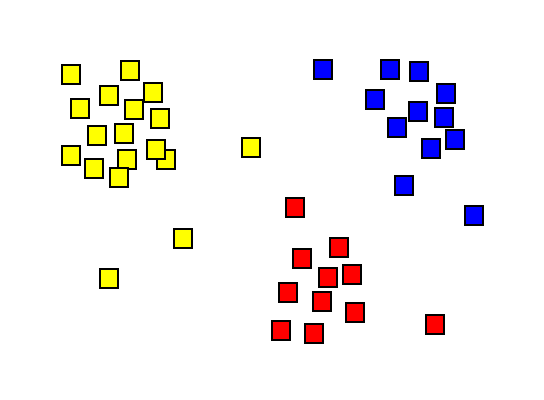
\includegraphics[width=0.35\linewidth]{fig/cluster.png}
    \caption{ตัวอย่างของชุดข้อมูลที่ถูกจัดกลุ่มโดยแบ่งตามสี}
    \label{fig:cluster}
\end{figure}

เทคนิค Clustering นั้นเป็นการจัดกลุ่มข้อมูลที่ไม่เคยมีการจัดกลุ่มมาก่อน กล่าวคือถ้าหากเรามีชุดข้อมูลที่ไม่เคยถูกวิเคราะห์ก่อนซึ่งข้อมูลเหล่านั้นก็ผสมกันแบบมั่ว ๆ หรือไม่มีรูปแบบ เราสามารถแบ่งกลุ่มข้อมูลได้โดยพิจารณาจากลักษณะที่คล้ายกันของข้อมูล โดยจะนำข้อมูลที่มีลักษณะคล้ายกันมาอยู่กลุ่มเดียวกัน ส่วนข้อมูลที่มีลักษณะต่างออกไปก็ให้ไปอยู่อีกกลุ่มหนึ่ง การนำเทคนิคนี้ไปใช้คือจะไม่ใช่การหาผลลัพธ์ที่ต้องการวัดค่าความแม่นยำ แต่จะเป็นการหาความสัมพันธ์ของข้อมูลอีกรูปแบบหนึ่ง เช่น การจัดกลุ่มข้อมูลของสารประกอบเคมีอินทรีย์โดยใช้ความว่องไวในการเข้าทำปฏิกิริยา การจัดกลุ่มหมู่ฟังก์ชันจากประเภทของการเข้าทำปฏิกิริยา

%--------------------------
\subsection{การจัดกลุ่มแบบโครงสร้างลำดับชั้น}
\label{ssec:hierar_clustering}
\idxboth{การจัดกลุ่มแบบโครงสร้างลำดับชั้น}{Hierarchical Clustering}
%--------------------------

การจัดกลุ่มแบบโครงสร้างลำดับชั้นจะใช้ลักษณะของต้นไม้ในการแทนความเชื่อมโยงของข้อมูล เป็นเทคนิคที่เหมาะสำหรับข้อมูลที่มีลำดับชั้น เช่น อนุกรมวิธาน (Taxonomy) การแบ่งกลุ่มลักษณะนี้มี 2 ประเภท คือ ล่างขึ้นบน (Agglomerative) และ บนลงล่าง (Divisive) ดังนี้
%
\begin{itemize}[topsep=0pt,noitemsep]\setlength\itemsep{0.5em}
    \item Agglomerative ในขั้นตอนแรกข้อมูลแต่ละตัวในชุดข้อมูลนั้นนับเป็นหนึ่งกลุ่ม หลังจากนั้นทำการคำนวณหาค่าความใกล้ชิดของกลุ่มที่อยู่ใกล้กัน ซึ่งกลุ่มที่อยู่ใกล้กันก็จะถูกรวบกันเป็นหนึ่งกลุ่ม โดยวนทำเช่นนี้ไปเรื่อย ๆ จนกว่าจะได้กลุ่มข้อมูลเดียวในที่สุด

    \item Divisive เทคนิคนี้จะดำเนินการตรงกันข้ามกับ Agglomerative ในขั้นตอนแรกเริ่มจากกลุ่มใหญ่กลุ่มเดียว และแยกกลุ่มที่ไม่เหมือนกันออกไปเรื่อย ๆ จนกระทั่งได้จำนวนกลุ่มเท่ากับจำนวนข้อมูลหรือจนกว่าจะแยกต่อไม่ได้
\end{itemize}

นอกจากนี้ยังมีเทคนิคการจัดกลุ่มข้อมูลแบบอื่นอีกที่ไม่ได้กล่าวถึง เช่น Centroid-based Clustering ใช้จุดกึ่งกลางของกลุ่ม, Density-based Clustering ใช้ความหนาแน่นหรือความแออัดของข้อมูล และ Distribution-based Clustering ใช้รูปแบบการแจกแจงของข้อมูล

%--------------------------
\subsection{วิธีรวบกลุ่มจับคู่แบบถ่วงน้ำหนักโดยใช้ค่าเฉลี่ยเลขคณิต}
\label{ssec:wpgma}
\idxboth{วิธีรวบกลุ่มจับคู่แบบถ่วงน้ำหนักโดยใช้ค่าเฉลี่ยเลขคณิต}{Weighted Pair Group Method with Arithmetic Mean}
%--------------------------

วิธีรวบกลุ่มจับคู่แบบถ่วงน้ำหนักโดยใช้ค่าเฉลี่ยเลขคณิต (Weighted Pair Group Method with Arithmetic Mean หรือ WPGMA) เป็นเทคนิคการจัดกลุ่ม (Clustering) แบบหนึ่งของวิธีโครงสร้างลำดับชั้น (Hierarchical Method) ซึ่งพัฒนาขึ้นมาโดยใช้ Pairwise Similarity Matrix\autocite{sokal1958} โดยนักชีววิทยาเชิงสถิติ Robert Reuven Sokal และนักกีฏวิทยา Robert Reuven Sokal

WPGMA เริ่มต้นด้วยการสร้างเดนโดรแกรม (Dendrogram)\footnote{เดนโดรแกรมคือแผนผังต้นไม้ ถูกใช้อย่างแพร่หลายในการวิเคราะห์แบบกลุ่มชีววิทยาเชิงคำนวณหรือชีวสารสนเทศศาสตร์} ซึ่งจะแสดงโครงสร้างของ Pairwise Similarity Matrix โดยในแต่ละสเต็ป กลุ่ม $i$ และกลุ่ม $j$ จะถูกจับรวมกันเป็นกลุ่มที่อยู่ในระดับที่สูงขึ้น หลังจากนั้นเราจะทำการคำนวณระยะห่างระหว่างกลุ่มที่เราสนใจกับกลุ่ม $k$ ซึ่งจะใช้ระยะห่างแบบค่าเฉลี่ยเลขคณิต (Airthmetic Mean) ระหว่างสมาชิกภายในกลุ่ม $k$ กับกลุ่ม $i$ และระยะห่างระหว่างสมาชิกกลุ่ม $k$ กับกลุ่ม $j$ ดังนี้
%
\begin{equation}\label{eq:wpgma}
    d_{(i \cup j),k} = \frac{d_{i,k} + d_{j,k}}{2}
\end{equation}

%--------------------------
\section{การแบ่งกลุ่มข้อมูลแบบเคมีน}
\label{sec:k_means}
\idxen{K-means Clustering}
%--------------------------

การแบ่งกลุ่มข้อมูลแบบเคมีน (K-means Clustering) เป็นหนึ่งในวิธีการแบ่งเวกเตอร์ซึ่งจะเป็นการแบ่งชุดข้อมูลที่มี $n$ ข้อมูลออกเป็น $k$ กลุ่ม ซึ่งเทคนิคนี้ได้ถูกใช้มาอย่างยาวนานตั้งแต่ในช่วงยุคเริ่มต้นของการทำ Data Mining\autocite{macqueen1967}

\begin{figure}[H]
    \centering
    \begin{subfigure}{0.4\textwidth}
        \centering
        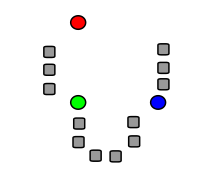
\includegraphics[width=0.5\linewidth]{fig/k-means-step1.png}
        \caption{เลือกค่าเฉลี่ย}
        \label{fig:k_means_step1}
    \end{subfigure}%
    \begin{subfigure}{0.4\textwidth}
        \centering
        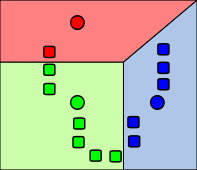
\includegraphics[width=0.5\linewidth]{fig/k-means-step2.png}
        \caption{สร้างคลัสเตอร์ k กลุ่ม}
        \label{fig:k_means_step2}
    \end{subfigure}
    \\
    \vspace{1em}
    \begin{subfigure}{0.4\textwidth}
        \centering
        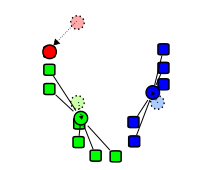
\includegraphics[width=0.5\linewidth]{fig/k-means-step3.png}
        \caption{คำนวณค่าเฉลี่ยใหม่}
        \label{fig:k_means_step3}
    \end{subfigure}%
    \begin{subfigure}{0.4\textwidth}
        \centering
        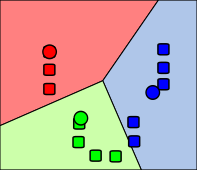
\includegraphics[width=0.5\linewidth]{fig/k-means-step4.png}
        \caption{ทำซ้ำจนกระทั่งค่ากลางลู่เข้า}
        \label{fig:k_means_step4}
    \end{subfigure}
    \caption{ขั้นตอนการทำ K-means Clustering (เครดิตภาพ: \url{https://en.wikipedia.org/wiki/K-means_clustering})}
    \label{fig:k_means}
\end{figure}

ภาพที่ \ref{fig:k_means} แสดงอัลกอริทึมของ K-means Clustering ที่มี 4 ขั้นตอน โดยขั้นตอนที่หนึ่งจะเป็นเลือกค่าเฉลี่ยเริ่มต้น $k$ (ในกรณีนี้ $k = 3$) แบบสุ่มจากโดเมนข้อมูล ขั้นตอนที่สองเป็นการสร้างคลัสเตอร์ $k$ กลุ่มรอบ ๆ ค่าเฉลี่ยทีได้กำหนดไว้โดยการเชื่อมโยงทุกข้อมูลการสังเกตด้วยค่าเฉลี่ยที่ใกล้ที่สุด (สังเกตระยะห่างระหว่างจุดวงกลมในแต่ละคลัสเตอร์ไปจนถึงเส้นแบ่ง) เส้นแบ่งในที่นี้แสดงให้เห็นแผนภาพของโวโรนอย (Voronoi Diagram) ที่สร้างขึ้นจากค่าเฉลี่ย ขั้นตอนที่สามคือคำนวณจุดศูนย์กลางหรือจุดเซนทรอยด์ (Centroid) ของโวโรนอยของแต่ละคลัสเตอร์และทำการกำหนดเป็นค่าเฉลี่ยค่าใหม่ ขั้นตอนที่สี่จะเป็นการทำสามขั้นตอนแรกซ้ำ ซึ่งจะทำซ้ำไปเรื่อย ๆ จนกว่าค่ากลางของแต่ละคลัสเตอร์จะไม่เปลี่ยนแปลง โดยเมื่อค่ากลางลู่เข้าแล้ว เราจะได้ฟังก์ชันที่มีเส้นแบ่งสำหรับการนำไปจัดคลัสเตอร์ของข้อมูล Test Set ต่อไป

หัวข้อถัดไปคือวิธีการลดขนาดมิติของข้อมูลแบบเชิงเส้นซึ่งผู้เขียนขออธิบาย 2 วิธี คือ การวิเคราะห์องค์ประกอบหลัก (Principal Component Analysis หรือ PCA) และ การสเกลแบบหลายมิติ (Multidimensional Scaling หรือ MDS)

%--------------------------
\section{การวิเคราะห์องค์ประกอบหลัก}
\label{sec:pca}
\idxboth{การวิเคราะห์องค์ประกอบหลัก}{Principal Component Analysis}
%--------------------------

การวิเคราะห์องค์ประกอบหลัก (Principal Component Analysis หรือ PCA) เป็นวิธีทางสถิติสำหรับการจัดกลุ่มตัวแปร ถูกนำมาใช้เพื่อรับมือกับข้อมูลที่มีจำนวนหลายมิติหรือมีหลายตัวแปร วิธี PCA ถูกพัฒนาโดยนักคณิตศาสตร์และชีววิทยาเชิงสถิติชาวอังกฤษ Karl Pearson โดยเทคนิค PCA สามารถหาความสัมพันธ์ของตัวแปรเหล่านั้นโดยทำการลดขนาดของมิติโดยสร้างชุดข้อมูลใหม่ที่อาศัยแกนอ้างอิงจากชุดข้อมูลเดิม ซึ่งจำนวนมิติที่ถูกลดลงนั้นก็มีจำนวนมิติเพียง 2 หรือ 3 มิติเท่านั้น ซึ่งทำให้ง่ายต่อการตีความและวิเคราะห์ข้อมูล เช่น การจัดกลุ่มชุดข้อมูลโดยจำแนกตาม Feature ซึ่ง Feature แต่ละคู่จะมีคุณสมบัติ Orthogonality หรือตั้งฉากกันนั่นเอง ทำให้เราสามารถแสดงผลลัพธ์ของ PCA ออกมาได้ในปริภูมิทั่วไป\footnote{\url{https://en.wikipedia.org/wiki/Principal_component_analysis}}

\begin{figure}[H]
    \centering
    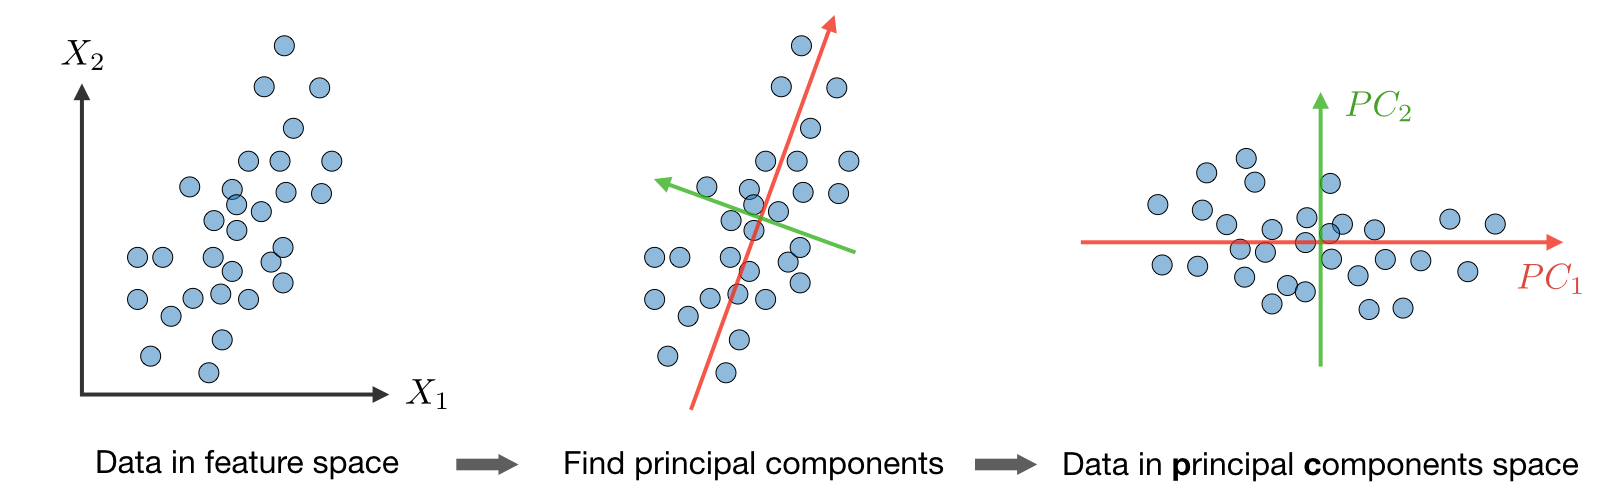
\includegraphics[width=\linewidth]{fig/pca_process.png}
    \caption{ขั้นตอนการทำ Principal Component Analysis ซึ่งเป็นการทำให้ค่าความแปรปรวน (Variance) ของข้อมูลนั้นมีค่ามากที่สุดในปริภูมิที่มี $k$ มิติ}
    \label{fig:pca_process}
\end{figure}

การทำ PCA ประกอบไปด้วยขั้นตอนดังต่อไปนี้
%
\begin{enumerate}[topsep=0pt,noitemsep]\setlength\itemsep{0.5em}
    \item Normalize ข้อมูลทั้งหมดเพื่อให้มีค่าเฉลี่ยเลขคณิต (Mean) หรือ $\mu$ เท่ากับ 0 และมีส่วนเบี่ยงเบนมาตรฐาน (Standard Deviation) หรือ $\sigma$ เท่ากับ 1 ซึ่งสามารถทำได้โดยการนำข้อมูลไปลบออกด้วย $\mu$ แล้วหารด้วย $\sigma$

          \begin{equation}\label{eq:normalize}
              x^{(i)}_{j} \leftarrow \frac{x^{(i)}_{j} - \mu_{j}}{\sigma_{j}}
          \end{equation}

          \noindent โดยที่ $\mu$ และ $\sigma$ สามารถหาได้ดังนี้

          \begin{equation}\label{eq:mean}
              \mu_{x} = \frac{1}{n} \sum^{n}_{i=1}(x_{i})
          \end{equation}

          \noindent และ

          \begin{equation}\label{eq:variance}
              \sigma^2_{x} = \frac{1}{n} \sum^{n}_{i=1}(x_{i} - \mu)^2
          \end{equation}

          \noindent นอกจากนี้เรายังสามารถหา Covariance ระหว่าง 2 ตัวแปรได้ดังนี้

          \begin{equation}\label{eq:covariance}
              \sigma(x, y) = \frac{1}{n-1} \sum^{n}_{i=1}{(x_i - \mu_{x})(y_i - \mu_{y})}
          \end{equation}

    \item คำนวณ Covariance Matrix $\Sigma$ ซึ่งมีความสมมาตรกับค่าไอเกนจริง (Real Eigenvalue) โดยมีนิยามดังต่อไปนี้

          \begin{equation}
              \Sigma = \frac{1}{n} \sum^{n}_{i=1}{(X_i-\bar{X})(X_i-\bar{X})^T}
          \end{equation}

          \noindent สำหรับกรณีแบบที่ง่ายที่สุดเราสามารถพิจารณา Covariance Matrix ของ 2 มิติ ดังนี้

          \begin{equation}\label{eq:cov_mat_2d}
              C = \left( \begin{array}{ccc}  \sigma(x, x) & \sigma(x, y) \\
             \sigma(y, x)        & \sigma(y, y)\end{array} \right)
          \end{equation}

    \item คำนวณค่าไอเกน (Eigenvalue) และเวกเตอร์ไอเกน (Eigenvector) ของ Covariance Matrix หลังจากนั้นเราจะทำการตัดสินใจเลือกว่าเราจะเก็บแกนไหนไว้บ้าง ซึ่งเราจะมาทำการเลือก Eigenvector นั่นเอง โดยเราจะทำการสร้าง Feature Vectors ซึ่งเป็นเมทริกซ์โดยมีคอลัมน์เป็น Eigenvector ที่เราจะเลือกว่าจะเก็บไว้โดยมาตรวจสอบค่าความสำคัญ (Significance) ของแต่ละ Eigenvector โดยดูที่ค่า Eigenvalue ถ้าหากว่ามี Eigenvalue น้อยก็หมายความว่ามี Significance ที่น้อย ซึ่งหลังจากที่เราได้ Feature Vectors แล้วเราจะนำไปใช้ในขั้นตอนต่อไป
    \idxboth{ค่าไอเกน}{Eigenvalue}
    \idxboth{เวกเตอร์ไอเกน}{Eigenvector}

    \item ขั้นตอนสุดท้ายคือแปลงตำแหน่งของข้อมูลโดยการเปลี่ยนแกน กล่าวคือขั้นตอนก่อนหน้านี้นั้นเราไม่ได้แก้ไขข้อมูลเลย (ยกเว้นแค่การทำ Standardization) โดยเราทำแค่การเลือกองค์ประกอบหลัก (Principal Components) แล้วก็สร้าง Feature Vector เท่านั้นเอง ดังนั้นข้อมูลจะยังคงอ้างอิงกับแกนเดิมอยู่ โดยในขั้นตอนนี้เราจะทำการ Projection ข้อมูลลงบนแกนใหม่ซึ่งเป็น Principal Components ที่ได้จาก Feature Vectors ซึ่งทำได้โดยการนำเมทริกซ์สลับเปลี่ยนของข้อมูลเดิมคูณกับเมทริกซ์สลับเปลี่ยน (Transpose Matrix) ของ Feature Vector

\end{enumerate}

%--------------------------
\section{การสเกลแบบหลายมิติ}
\label{sec:mds}
\idxboth{การสเกลแบบหลายมิติ}{Multidimensional Scaling}
%--------------------------

การสเกลแบบหลายมิติ (Multidimensional Scaling หรือ MDS)\autocite{young1938,torgerson1952}

สำหรับวิธีการลดขนาดมิติของข้อมูลแบบเชิงเส้นนั้นไม่ซับซ้อนและมีจำนวนวิธีที่ไม่มาก แต่ในกรณีของวิธีการลดขนาดมิติแบบไม่เชิงเส้นนั้นจะซับซ้อนมากกว่า โดยมีอัลกอริทึมที่ถูกพัฒนาแตกต่างกันไปตามหัวข้อย่อยต่อไปนี้\autocite{glielmo2021}
%
\begin{itemize}[topsep=0pt,noitemsep]\setlength\itemsep{0.5em}
    \item Isometric Feature Mapping (Isomap)

    \item Kernel PCA

    \item Diffusion Map

    \item Sketch-Map (ไม่ได้ลงรายละเอียด)
\end{itemize}

%--------------------------
\section{การเชื่อมโยงลักษณะเฉพาะแบบไอโซเมตริก}
\label{sec:isomap}
\idxboth{การเชื่อมโยงลักษณะเฉพาะแบบไอโซเมตริก}{Isometric Feature Mapping}
%--------------------------

การเชื่อมโยงลักษณะเฉพาะแบบไอโซเมตริก (Isometric Feature Mapping หรือ Isomap)\autocite{tenenbaum2000} ถูกพัฒนาขึ้นมาเพื่อแก้ปัญหาที่เรามักจะพบเมื่อเราใช้วิธีการลดจำนวนมิติของข้อมูลแบบเส้นตรง เช่น วิธี PCA ซึ่งไม่สามารถหาตำแหน่งของข้อมูลที่ถูกต้องได้ ไอเดียของ Isomap ก็คือการสร้าง Representation ที่อยู่ในมิติต่ำ ๆ ที่สามารถรักษาหรือคงไว้ซึ่งระยะห่างแบบจีโอดีซิค (Geodesic Distance) ระหว่างจุดข้อมูลซึ่งเป็นระยะทางที่สั้นที่สุดบนทรงรี แทนที่จะใช้ระยะห่างแบบคาร์ทีเซียน (Cartesian Distance) ตัวอย่างแสดงตามภาพที่ \ref{fig:map_geodesic_euclidean} โดยโลกของเราคือ Manifold และประเทศสวิตเซอร์แลนด์กับสโลวีเนียคือจุดของข้อมูล

\begin{figure}[H]
    \centering
    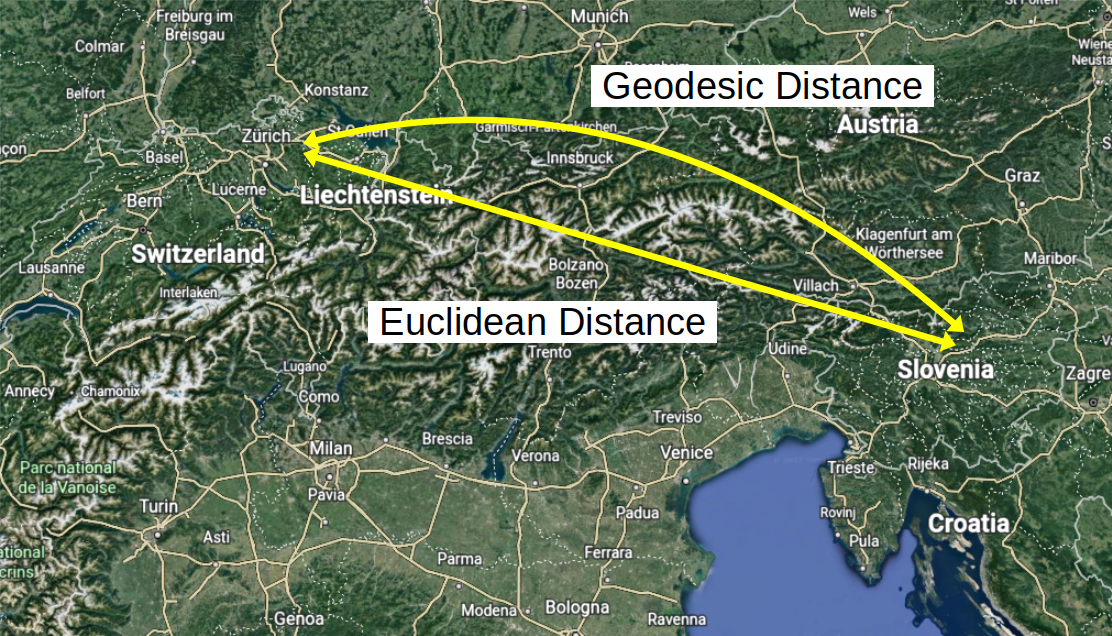
\includegraphics[width=0.75\linewidth]{fig/map_geodesic_euclidean.png}
    \caption{แสดงระยะห่างแบบ Euclidean และ Geodesic ระหว่างประเทศสวิตเซอร์แลนด์และสโลวีเนีย}
    \label{fig:map_geodesic_euclidean}
\end{figure}

การทำ Isomap ประกอบไปด้วย 3 ขั้นตอนดังนี้
%
\begin{enumerate}[topsep=0pt,noitemsep]\setlength\itemsep{0.5em}
    \item สร้างกราฟโดยใช้ข้อมูลที่เป็นแบบ Local Connectivities ซึ่งในกราฟอันนี้จุดข้อมูลแต่ละจุดจะถูกเชื่อมโยงไปยังจุดที่ใกล้ที่สุด (\textit{k}th Nearest Neighbor) ซึ่งถูกคำนวณด้วยระยะห่างของคู่ของข้อมูล (Pairwise Distance)

    \item คำนวณหาระยะห่างที่สั้นที่สุดของข้อมูลทุกคู่ในกราฟโดยสามารถใช้การประมาณค่าระยะห่างแบบย่อย ๆ ได้ ตามภาพที่
          \ref{fig:approx_geodesic}

          \begin{figure}[H]
              \centering
              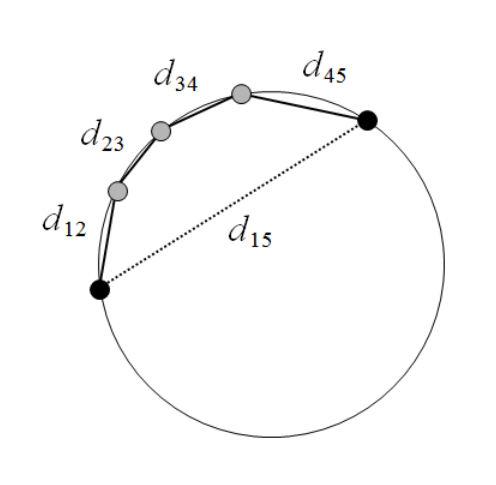
\includegraphics[width=0.3\linewidth]{fig/approx_geodesic.png}
              \caption{การประมาณค่าระยะห่างแบบ Geodesic}
              \label{fig:approx_geodesic}
          \end{figure}

    \item นำเมทริกซ์ $R_{ij}$ มาทำ Multidimensional Scaling ซึ่งเมทริกซ์นี้จะเก็บข้อมูล Geodesic Distance ของข้อมูลแต่ละคู่ไว้
\end{enumerate}

%--------------------------
\section{การวิเคราะห์องค์ประกอบหลักแบบเคอร์เนล}
\label{sec:kernel_pca}
\idxboth{การวิเคราะห์องค์ประกอบหลักแบบเคอร์เนล}{Kernel PCA}
%--------------------------

วิธีต่อมาที่ได้รับความนิยมเช่นเดียวกันคือการวิเคราะห์องค์ประกอบหลักแบบเคอร์เนล (Kernel PCA)\autocite{scholkopf1998} ซึ่งเป็นวิธีที่ถูกใช้สำหรับการหา Low-dimensional Representation เช่นเดียวกันแต่ว่ามีประสิทธิภาพมากเมื่อนำมาใช้กับข้อมูลที่เป็นถูกมองเป็น Manifold แบบที่เป็นเส้นโค้ง (Curved) หรือบิดเบี้ยวไป (Twisted) โดยใน Kernel PCA นั้นจริง ๆ แล้วไม่ได้ทำการแปลงข้อมูล (Transformation) โดยตรงแต่ว่าทำอ้อม ๆ ผ่านฟังก์ชันเคอร์เนล $K(x,x')$ ในกรณีที่เราใช้ฟังก์ชันเคอร์เนลเป็นแบบเชิงเส้น (Linear Kernel) เช่น
%
\begin{equation}
    K(x_{i},x_{j}) = x^{T}_{i}x_{j}
\end{equation}
%
\noindent จะทำให้ Kernel PCA กลายเป็น PCA แบบมาตรฐานทั่วไป ดังนั้นการที่เราเปลี่ยนไปใช้ฟังก์ชันเคอร์เนลแบบพหุนาม (Polynomial Kernel) ดังนี้
%
\begin{equation}
    K(x_{i},x_{j}) = (x^{T}_{i}x_{j})^{p}
\end{equation}
%
\noindent จะสามารถเพิ่มขนาดของ Feature Space ได้ตามขนาดของค่าดีกรี $p$

%--------------------------
\section{วิธีแผนที่แบบแพร่กระจาย}
\label{sec:diff_map}
\idxboth{วิธีแผนที่แบบแพร่กระจาย}{Diffusion Map}
%--------------------------

วิธีแผนที่แบบแพร่กระจาย (Diffusion Map)\autocite{coifman2005,coifman2006} เป็นอีกเทคนิคหนึ่งที่มีความคล้ายกับ Kernel PCA เพราะว่าเป็นวิธีที่สามารถใช้ในการหาตัวแปรแบบไม่เป็นเส้นตรง (Nonlinear Variables) ที่สามารถอธิบายระบบของเรา (ชุดข้อมูล) ได้ในปริภูมิที่มีจำนวนมิติต่ำ ๆ โดยเราสามารถประยุกต์ใช้ Diffusion Map ในการวิเคราะห์ Trajectory\footnote{Trajectory (แปลเป็นไทยว่า วิธี) คือการเก็บข้อมูล Configuration ของโมเลกุลที่เปลี่ยนแปลงไปตามเวลาที่ใช้ในการจำลองด้วยคอมพิวเตอร์} ที่ได้จากการคำนวณ Molecular Dynamics ได้

\begin{figure}[H]
    \centering
    \begin{subfigure}{0.5\textwidth}
        \centering
        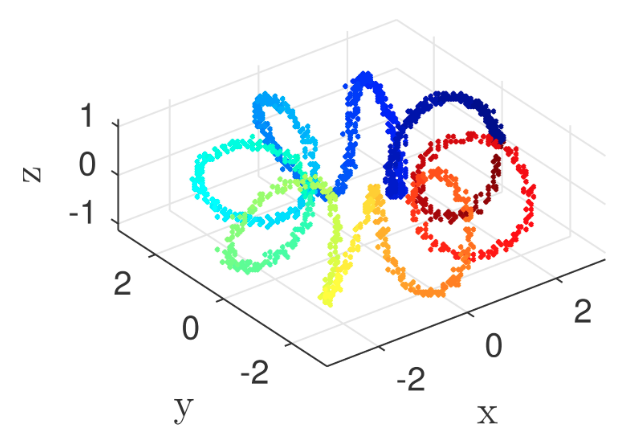
\includegraphics[width=0.7\linewidth]{fig/diff_map-1.png}
        \caption{ข้อมูลที่มีการกระจายอย่างไม่สม่ำเสมอบนเกลียวแบบวงแหวน (Toroidal Helix)}
        \label{fig:diff_map_1}
    \end{subfigure}%
    \begin{subfigure}{0.5\textwidth}
        \centering
        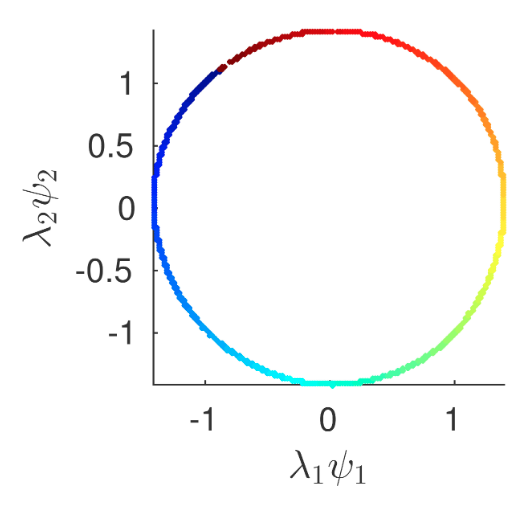
\includegraphics[width=0.7\linewidth]{fig/diff_map-2.png}
        \caption{พิกัดของ Diffusion Map 2 อันดับแรกซึ่งมีการทำ Normalization โดยใช้เทคนิค Laplace-Beltrami Normalization ด้วย}
        \label{fig:diff_map_2}
    \end{subfigure}
    \caption{Diffusion Map (เครดิตภาพ: \url{https://en.wikipedia.org/wiki/Diffusion_map})}
\end{figure}
\idxth{วิธีแผนที่แบบแพร่กระจาย!เกลียวแบบวงแหวน}
\idxen{Diffusion Map!Toroidal Helix}

ในการคำนวณ Diffusion Map นั้น เราจะเริ่มต้นด้วยการคำนวณ Gaussian Kernel
%
\begin{equation}
    K(x_{i}, x_{j}) = \exp \left( -\frac{||x_i-x_j||^2}{2\sigma^2} \right)
\end{equation}
%
\noindent ซึ่งเป็นฟังก์ชันเคอร์เนลอันเดียวกันกับสมการที่ \eqref{eq:gaussian_kernel} แต่ว่าสิ่งที่ทำให้ Diffusion Map นั้นแตกต่างไปจากวิธีเคอร์เนลทั่วไปก็คือในเทคนิคจะมีการประมาณค่าฟังก์ชันไอเกน (Eigenfunction) ที่ชื่อว่าโอเปอเรเตอร์ฟอกเกอร์-พลังค์ (Fokker-Planck Operator) สำหรับการทำ Diffusion Process\autocite{trstanova2020} โดยเราจะต้องมีการปรับฟังก์ชันเคอร์เนลโดยการทำให้เป็นปกติ (Normalization)\autocite{nadler2006} ตามสมการต่อไปนี้
\idxboth{ฟังก์ชันไอเกน}{Eigenfunction}
\idxboth{โอเปอเรเตอร์ฟอกเกอร์-พลังค์}{Fokker-Planck Operator}
%
\begin{equation}
    \tilde{K}_{ij} = \frac{K_{ij}}{\sqrt{\sum_{k}K_{jk} \sum_{s}K_{js}}}
\end{equation}
%
\noindent แล้วตามด้วยการคำนวณเมทริกซ์การเปลี่ยนแปลง (Transition Matrix) ของ Diffusion Map ดังนี้
\idxboth{เมทริกซ์การเปลี่ยนแปลง}{Transition Matrix}
%
\begin{equation}
    P_{ij} = \frac{\tilde{K}_{ij}}{\sum_{j}\tilde{K}_{ij}}
\end{equation}
%
\noindent ซึ่งผลลัพธ์ที่ได้นั้น $P_{ij}$ คือความน่าจะเป็นของการเปลี่ยนแปลง (Transition Probability) จากข้อมูลที่ $i$ ไปยังข้อมูลที่ $j$ ซึ่งผลรวมของ Proability ในการเปลี่ยนแปลงไปยังข้อมูลหนึ่ง ๆ นั้น $(\sum_{j}P_{ij})$ จะต้องมีค่าเท่ากับ 1 \idxboth{ความน่าจะเป็นของการเปลี่ยนแปลง}{Transition Probability}

เมื่อเราได้ $P_{ij}$ ขั้นตอนต่อไปที่เราสามารถคำนวณได้ก็คือ Stochastic Matrix ซึ่งมีคุณสมบัติหลาย ๆ อย่างที่น่าสนใจเช่นเดียวกันแต่ว่าผู้เขียนไม่ขอลงรายละเอียด

%--------------------------
\section{การเข้ารหัสแบบอัตโนมัติ}
\label{sec:autoencoder}
\idxboth{การเข้ารหัสแบบอัตโนมัติ}{Autoencoder}
%--------------------------

\begin{figure}[H]
    \centering
    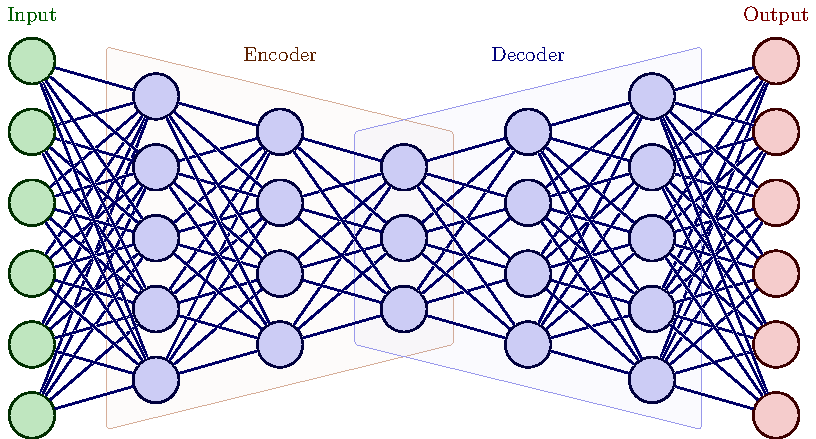
\includegraphics[width=0.7\linewidth]{fig/autoencoder.pdf}
    \caption{โครงข่ายประสาทของ Autoencoder ที่มีลักษณะความเป็นสมมาตร}
    \label{fig:autoencoder}
\end{figure}

ตัวเข้ารหัสแบบอัตโนมัติ (Autoencoder หรือ AE)\autocite{kramer1991} เป็นอัลกอริทึม Unsupervised Learning แบบหนึ่งที่ใช้โมเดล ANN โดยมีรูปแบบของโครงข่าย (Network) ที่เฉพาะตัวนั่นก็คือจะทำการลดมิติของข้อมูลโดยทำการบีบอัดข้อมูลหรือเข้ารหัส (Encoding) หรือ $E$ และทำการถอดรหัส (Decoding) ออกมาเป็นข้อมูลเดิม\autocite{ballard1987} ผ่านตัวถอดรหัส (Decoder) หรือ $D$
%
\begin{equation}\label{eq:encoder}
    y = E(x)
\end{equation}
%
\begin{equation}
    \tilde{x} = D(y)
\end{equation}
%
\noindent โดยที่ $x$, $y$ และ $\tilde{x}$ คือข้อมูลอินพุต ข้อมูลเอาต์พุต และข้อมูลอินพุตที่ถูกถอดรหัสออกมา ตามลำดับ

ตัวโมเดล AE มีความพิเศษคือจะมีลักษณะของความสมมาตรและมีความแตกต่างจาก PCA นั่นก็คือสามารถบีบอัดหรือลดจำนวนมิติของข้อมูลแบบไม่เป็นเส้นตรงได้ (Nonlinear) ได้ด้วยการใช้ฟังก์ชันกระตุ้นแบบ Nonlinear

\noindent ตัวอย่างการเขียนโค้ดของ Autoencoder ด้วย TensorFlow มีดังต่อไปนี้

\begin{lstlisting}[style=MyPython]
import tensorflow as tf

from tensorflow.keras import layers, losses
from tensorflow.keras.models import Model

latent_dim = 64 

class Autoencoder(Model):
    def __init__(self, latent_dim):
        super(Autoencoder, self).__init__()
        self.latent_dim = latent_dim   
        self.encoder = tf.keras.Sequential([
            layers.Flatten(),
            layers.Dense(latent_dim, activation='relu'),
        ])
        self.decoder = tf.keras.Sequential([
            layers.Dense(784, activation='sigmoid'),
            layers.Reshape((28, 28))
        ])

    def call(self, x):
        encoded = self.encoder(x)
        decoded = self.decoder(encoded)
        return decoded

autoencoder = Autoencoder(latent_dim)
autoencoder.compile(optimizer='adam', 
                    loss=losses.MeanSquaredError())
autoencoder.fit(x_train, x_train,
                epochs=10,
                shuffle=True,
                validation_data=(x_test, x_test))
\end{lstlisting}

\vspace{1em}

\noindent จริง ๆ แล้ว Autoencoder แบบทั่วไปนั้นก็คือ Neural Network แบบง่ายที่มีจำนวนและขนาดของ Hidden Layer ที่สมมาตรกัน
